\documentclass{beamer}

\usepackage[utf8]{inputenc}


%Information to be included in the title page:
\title{MTH 201: Calculus}
\subtitle{Module 3A: Interpreting, estimating, and using the first and second derivatives}
\author{Prof. Talbert}
\institute{GVSU}
\date{\today}


\begin{document}

\frame{\titlepage}

\begin{frame}{Agenda for today}
    \begin{itemize}
        \item<1-> Review of Daily Prep assignment, and Q+A
        \item<2-> Polling activity:Increasing/decreasing behavior, meaning of the derivative, concavity
        \item<3-> Lecture: Connecting concave up/down to the first and second derivatives 
        \item<4-> Followup activities and things to do 
    \end{itemize}
\end{frame}

\begin{frame}
    \frametitle{Review and Q+A}

    \begin{center}
        Go to \url{www.menti.com} and use code \texttt{?}
    \end{center}

\end{frame}

\begin{frame}
    \frametitle{Concavity}

    \begin{block}{Definition: Concave up}
        A function $f$ is \textbf{concave up} on an interval if

        \begin{itemize}
            \item $f$ is either increasing or decreasing at an increasing rate on the interval
            \item The graph of $f$ sits above its tangent lines on the interval
            \item $f'$ is increasing on the interval
        \end{itemize}
    \end{block}

\begin{center}
    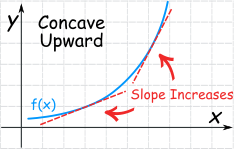
\includegraphics[width=2in]{concave-upward.png}
\end{center}


\end{frame}


\begin{frame}
    \frametitle{Concavity}

    \begin{block}{Definition: Concave down}
        A function $f$ is \textbf{concave \alert{down}} on an interval if

        \begin{itemize}
            \item $f$ is either increasing or decreasing at an \alert{decreasing} rate on the interval
            \item The graph of $f$ sits \alert{below} its tangent lines on the interval
            \item $f'$ is \alert{decreasing} on the interval
        \end{itemize}
    \end{block}

\begin{center}
    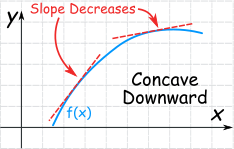
\includegraphics[width=2in]{concave-downward.png}
\end{center}


\end{frame}

\begin{frame}
    \frametitle{Four combinations of behaviors}

    \begin{center}
        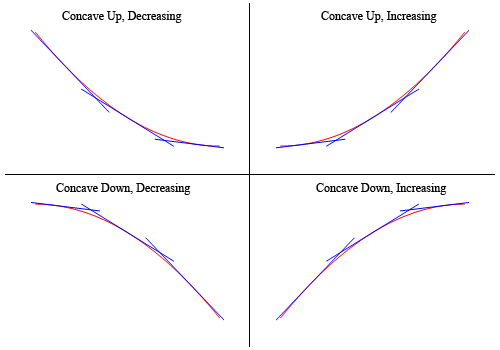
\includegraphics[width=4in]{behavior-combos.png}
    \end{center}

\end{frame}

\begin{frame}
    \frametitle{Identifying concavity}

    \begin{center}
        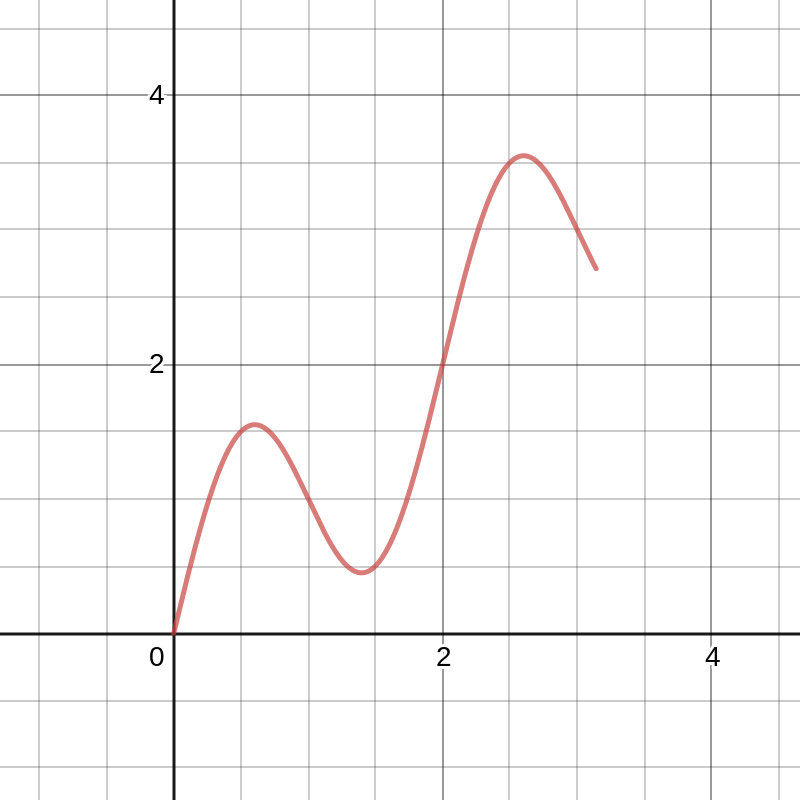
\includegraphics[width=3in]{concavity.png}
    \end{center}

\end{frame}

\begin{frame}
    \frametitle{The second derivative}

    \begin{block}{The second derivative}
        The \textbf{second derivative} of a function $f$ is the derivative of its derivative. \\
        Notation: $f''(x)$ or $\displaystyle{\frac{d^2y}{dx^2}}$
    \end{block}

    The second derivative tells you \textbf{the rate at which the slopes of $f$ are changing} \\

    Or, \textbf{whether $f'$ is increasing or decreasing}

\end{frame}

\begin{frame}
    \frametitle{Connecting some pieces}

    \begin{itemize}
        \item<1-> $f$ is concave up if $f'$ is increasing 
        \item<2-> $f'$ is increasing if the derivative of $f'$ is positive 
        \item<3-> The derivative of $f'$ is $f''$
    \end{itemize} \pause

    \textbf{Therefore... $f$ is concave up if}

\end{frame}


\begin{frame}
    \frametitle{Next}

\textbf{All due dates are on the Course Calendar}


    \begin{itemize}
        \item Complete Followup Activities
    \end{itemize}

\end{frame}
 
\end{document}